
%(BEGIN_QUESTION)
% Copyright 2006, Tony R. Kuphaldt, released under the Creative Commons Attribution License (v 1.0)
% This means you may do almost anything with this work of mine, so long as you give me proper credit

Identify the ``high'' and ``low'' ports on this pneumatic differential pressure transmitter, and explain your reasoning:

$$\includegraphics[width=15.5cm]{i00223x01.eps}$$

Also, explain how this transmitter will respond to an increasing pressure at each of its two ports, including the operation of the bellows feedback mechanism.

\underbar{file i00223}
%(END_QUESTION)





%(BEGIN_ANSWER)

Port ``A'' is the ``high'' pressure port on this transmitter, and port ``B'' is the ``low'' pressure port.  Remember: an increasing pressure applied to the ``high'' port causes an increasing signal out of the transmitter.  Conversely, an increasing pressure applied to the ``low'' port causes a decreasing signal out of the transmitter.

%(END_ANSWER)





%(BEGIN_NOTES)


%INDEX% Measurement, pressure: ``high'' versus ``low'' ports of a DP instrument

%(END_NOTES)


